%%%%%%%%%%%%%%% a place to park unused tex %%%%%%%%%%%%%

\begin{figure}[ht!]
  \centering
    \includegraphics[width=0.7\textwidth]{nonhexapod/scorpCCLXXXIX}
  \caption{Scorpiones \cite[][Plate CCLXXXIX]{bhlitem55834arach}}
  \label{fig:scorpion}
\end{figure}

\begin{figure}[ht!]
  \centering
\begin{subfigure}[ht!]{0.42\textwidth}
    \includegraphics[width=\textwidth]{coleopterida/LucanidHabitus2}
  \caption{}
  \label{fig:lucanid1}%need line drawing or black and white
\end{subfigure}
    \qquad
\begin{subfigure}[ht!]{0.47\textwidth}
    \includegraphics[width=\textwidth]{coleopterida/LucanidHabitus}
  \caption{}
  \label{fig:lucanid}\end{subfigure}%need line drawing or black and white - https://flic.kr/p/2krxdrX ... https://flic.kr/p/a6VKFr
    \caption{Lucanidae. Photos (CC BY-SA 2.0) by Udo Schmidt \textbf{(a)}  \url{https://flic.kr/p/fsYiJ2}; \textbf{(b)} \url{https://flic.kr/p/5CdfQj}}\label{fig:lucanids}
\end{figure}



\begin{figure}[ht!]
  \centering
\begin{subfigure}[ht!]{0.25\textwidth}
    \includegraphics[width=\textwidth]{ScarabHabitus1}
  \caption{}
  \label{fig:scarabaeid1}
\end{subfigure}
    ~
\begin{subfigure}[ht!]{0.25\textwidth}
    \includegraphics[width=\textwidth]{ScarabHabitus2}
  \caption{}
  \label{fig:scarabaeid2}
\end{subfigure}
    ~
\begin{subfigure}[ht!]{0.23\textwidth}
    \includegraphics[width=\textwidth]{ScarabHabitus4}
  \caption{}
  \label{fig:scarabaeid3}
\end{subfigure}
    \caption{Scarabaeidae. Photos (CC BY-SA 2.0) by Udo Schmidt \textbf{(a)}  \url{https://flic.kr/p/pSabdG}; \textbf{(b)} \url{https://flic.kr/p/pKYJEA}; \textbf{(c)}  \url{https://flic.kr/p/nqwaxk}}\label{fig:scarabaeids}
\end{figure}%need line drawing or black and white



\subsubsection*{Copepoda (copepods, fish lice)}\index{Copepoda}
What group does it belong in and why? What diagnostic characters separate it from the taxa above?\\

\noindent{}What do these arthropods eat, and how do they live?\vspace{2cm}

\begin{figure}[ht!]
  \centering
    \includegraphics[width=0.7\textwidth]{copepoda}
  \caption{Freshwater copepods. Modified from Figs. 285,286 in \cite{bhlitem155735cope}}
  \label{fig:copepod}
\end{figure}


\hangindent2em\textbf{Question 2:}  Based on the eye morphology and feeding habits of the preceding four families (2.1--2.4) what would you hypothesize about the natural history of Ascalaphinae?


\subsubsection{Coccidae (soft scale insects, wax and tortoise scales)}\index{Coccidae}
\noindent{}\textit{Diagnostic characters:} adult female flattened and oval with smooth, hard exoskeleton or soft waxy covering (Figure \ref{fig:coccid2}); antennae reduced or absent; legs often present but reduced; 2 triangular plates on anal opening; abdomen with anal cleft; abdominal spiracles absent.\\

\noindent{}\textit{Natural history:} Females smooth and dorso-ventrally flattened. More than 1,100 species have been described worldwide, including many economically important pests.\\

\begin{figure}[ht!]
 \centering
 \begin{subfigure}[ht!]{0.45\textwidth}
  \includegraphics[width=\textwidth]{CoccidDorsalHabitus}
  \caption{Dorsal habitus. Photo (CC BY 2.0) by Katja Schulz \url{https://flic.kr/p/qLWfyn}}
  \label{fig:coccid1}
 \end{subfigure}
 \qquad
 \begin{subfigure}[ht!]{0.45\textwidth}
  \includegraphics[width=\textwidth]{CoccidHabitus}
  \caption{Ventral habitus (image from \cite{ScaleNet})}
  \label{fig:coccid2}
 \end{subfigure}
 \caption{Coccidae}\label{fig:coccid}
\end{figure}


\subsubsection{Monophlebidae (giant scale insects)}\index{Monophlebidae}
\noindent{}\textit{Diagnostic characters:} adult female flattened or spherical, often cylindrical or scalloped, with hard covering formed of wax and cast skins of earlier instars; abdominal spiracles present; female antennae short or long, up to 13 segments, no wings or legs.\\

\noindent{}\textit{Natural history:} Approximately 240 species known worldwide, including the Cottony Cushion Scale (Icerya purchasi Maskell 1878), and important pest of many plants. Most species feed on trees or woody shrubs.\\

\begin{figure}[ht!]
 \centering
 \begin{subfigure}[ht!]{0.42\textwidth}
  \includegraphics[width=\textwidth]{MonophlebidDorsalHabitus}
  \caption{Dorsal habitus. Photo (CC BY-SA 3.0) by Lucarelli \url{https://goo.gl/dQNTNy}}
  \label{fig:monophlebid1}
 \end{subfigure}
 \qquad
 \begin{subfigure}[ht!]{0.45\textwidth}
  \includegraphics[width=\textwidth]{MonophlebidHabitus}
  \caption{Ventral habitus (image from \cite{ScaleNet})}
  \label{fig:monophlebid2}
 \end{subfigure}
 \caption{Monophlebidae}\label{fig:monophlebids}
\end{figure}


\subsubsection{Pseudococcidae (mealybugs)}\index{Pseudococcidae}
\noindent{}\textit{Diagnostic characters:} body ovular, usually with a powdery waxy coating; terminal abdominal segments, anal opening with setae; dorsal ostioles present; abdominal spiracles absent.\\

\noindent{}\textit{Natural history:} More than 2,200 species have been described worldwide, and they vary quite a bit morphologically. When alive they can often be recognized by their waxy, powdery appearance.\\

\begin{figure}[ht!]
 \centering
 \begin{subfigure}[ht!]{0.38\textwidth}
  \includegraphics[width=\textwidth]{pseudococcidae}
  \caption{Dorsal habitus; arrow = egg mass. Illustration by John Davidson, Department of Entomology, University of Maryland}
  \label{fig:pseudococcid1}
 \end{subfigure}
 \qquad
 \begin{subfigure}[ht!]{0.45\textwidth}
  \includegraphics[width=\textwidth]{PseudococcidHabitus}
  \caption{Ventral habitus (image from \cite{ScaleNet})}
  \label{fig:pseudococcid2}
 \end{subfigure}
 \caption{Pseudococcidae}\label{fig:pseudococcid}
\end{figure}


\subsubsection{Argidae (argid sawflies)}\index{Argidae}%drop this from sight ID? I think so
\noindent{}\textit{Diagnostic characters:} Antenna with 1 flagellomere, sometimes U-shaped (figure \ref{fig:argid1}); mesonotum not divided by straight transverse groove; fore wing 2r vein absent.\vspace{3mm}

\noindent{}\textit{Natural history:} Typically foliage feeders, this taxon is much more diverse in the tropics (\textgreater800 spp.) than in North America ($\sim$70 spp.)

\begin{figure}[ht!]
    \centering
    \begin{subfigure}[ht!]{0.11\textwidth}
        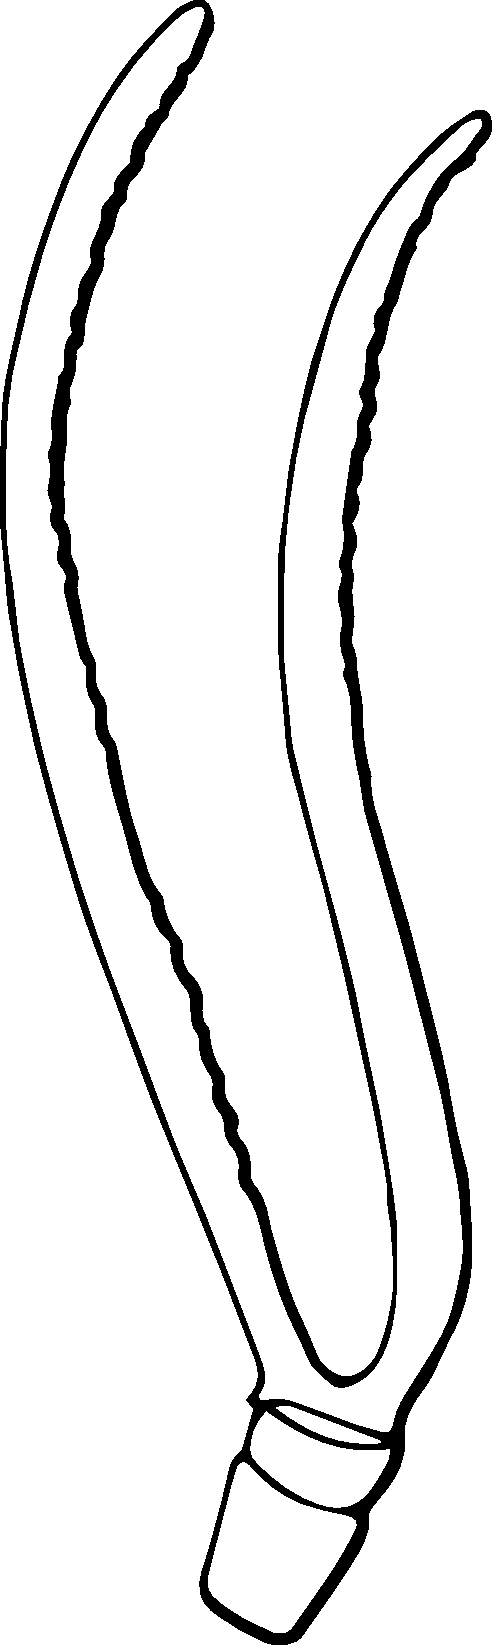
\includegraphics[width=\textwidth]{hymenoptera/ArgidAntenna}
        \caption{}
        \label{fig:argid1}
    \end{subfigure}
    \qquad
    \begin{subfigure}[ht!]{0.45\textwidth}
        \reflectbox{\includegraphics[width=\textwidth]{hymenoptera/ArgidHabitus}}
        \caption{Habitus}
        \label{fig:argid2}
    \end{subfigure}
    \caption{Argidae. \textbf{(a)} Antenna \citep[][pg. 106]{goulet1993hymenoptera}; \textbf{(b)} habitus \citep[][Fig. 26]{goulet1993hymenoptera}}\label{fig:argid}
\end{figure}

\subsubsection{Pipunculidae (big-headed flies)}\index{Pipunculidae}%drop this family?
\noindent{}\textit{Diagnostic characters:} CuA2 reaches wing margin or joins A1 near margin; R4+5 do not branch, C ends at wing apex; antennae aristate; head strongly hemispherical, eyes LARGE; usually small, black and shiny.\vspace{3mm}

\noindent{}\textit{Natural history:} Larvae develop almost exclusively as parasitoids of Auchenorrhyncha. About 1,200 spcie have been described worldwide.

\begin{figure}[ht!]
    \centering
    \begin{subfigure}[ht!]{0.45\textwidth}
        \includegraphics[width=\textwidth]{antliophora/PipunculidWing}
        \caption{}
        \label{fig:pipunculid1}
    \end{subfigure}
    \qquad
    \begin{subfigure}[ht!]{0.42\textwidth}
        \includegraphics[width=\textwidth]{antliophora/PipunculidHabitus}
        \caption{}
        \label{fig:pipunculid2}
    \end{subfigure}
    \caption{Pipunculidae. \textbf{(a)} Fore wing \citep[][Fig. 4.50]{mcalpine1981manual}; \textbf{(b)} habitus \citep[][Fig. 53.1]{mcalpine1981manualv2}}\label{fig:pipunculids}
\end{figure}

\subsubsection{Cleridae (checkered beetles)}\index{Cleridae}
\noindent{}\textit{Diagnostic characters:} Several tarsomeres lobed; fore coxa with exposed trochantin (small sclerite attached to coxa), coxae projecting ventrally, circular; hind coxa reaches elytra- ``open''; antennae sometimes clubbed, saw-toothed or threadlike; eye often emarginate; pronotum usually longer than wide; body elongate-narrow, pronotum and head narrower than elytra, hard-bodied often marked with colors and always bristly/hairy.\vspace{3mm}

\noindent{}\textit{Natural history:} Most clerid species are predators of other insects, although some are scavengers or pollen-feeders. Some species are important for controlling pestiferous bark beetles. About 3,500 species have been described worldwide.

\begin{figure}[ht!]
  \centering
\begin{subfigure}[ht!]{0.45\textwidth}
    \includegraphics[width=\textwidth]{coleopterida/CleridHabitus}
  \caption{}
\end{subfigure}
\hfill
\begin{subfigure}[ht!]{0.4\textwidth}
    \includegraphics[width=\textwidth]{coleopterida/CleridaeHead}
  \caption{}
  \end{subfigure}
    \caption{Cleridae. \textbf{(a)} Habitus (photo (CC BY-SA 2.0) by Udo Schmidt; \url{https://flic.kr/p/25pahvs}; (b) head and prothorax (photo (CC BY-SA 2.0) by Udo Schmidt;\url{https://flic.kr/p/pLAeE2})}\label{fig:clerid}
\end{figure}
